\section{La revue de code}
La revue de code représente une démarche que nous avions mis en avant dans le plan qualité. L'objectif visé est de tendre un projet dont l'intégralité du code a été revu. 

La revue de code se fait au moment de l'intégration, c'est pourquoi toutes intégrations nécessitent la création préalable d'une \PullRequest. Pour cela, une fois le travail correspondant à une \UserStory{} est fini\footnote{selon nos critères définis lors de la présentation de la méthode \Scrum{} \ref{methodeScrum}}, le développeur crée une \PullRequest{} via l'outil \Github. Il défini
\begin{figure}
	\centering
	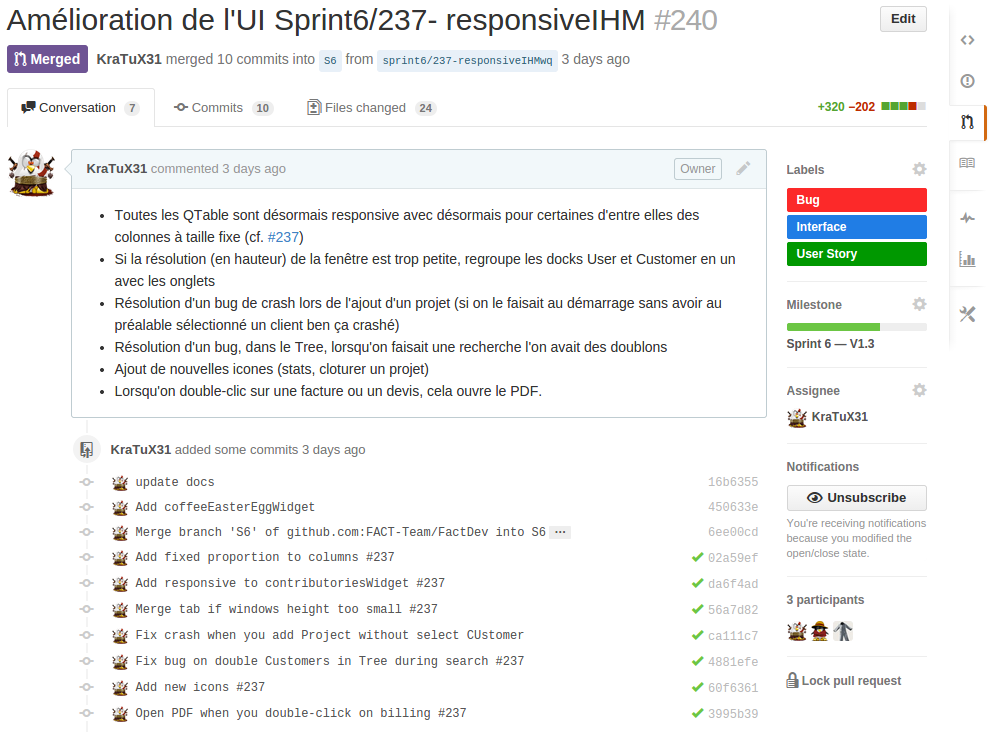
\includegraphics[width=0.7\linewidth]{screens/creation_pr_github}
	\caption{Exemple de \PullRequest{} du projet \FactDev}
	\label{fig:creation_pr_github}
\end{figure}

